\acused{dost2}\ac{dost2} ist der Name der zweiten internationalen
Friedenskonferenz nach dem Ausbruch des dritten Weltkriegs vor sieben-komma-drei
Jahren (März vor sieben Jahren).
Die erste Friedenskonferenz, \emph{Dost.-1.0}, fand zwei-komma-vier Jahre nach
Ausbruch des Krieges statt und hatte weitreichende Erfolge erzielt\footnote{
  Eines der zentralsten Ergebnisse war eine gemeinsame Erklärung, keine
  international noch kooperierenden Wirtschaftsstandorte anzugreifen, um nicht
  nur die beteiligten, sondern \emph{alle} Staaten vor einer wirtschaftlichen
  Depression zu schützen.
}.
Dass so lange keine weiteren Verhandlungen eines solches Ausmaßes mehr
stattgefunden hatten, war der Tatsache geschuldet, dass Staaten und Trusts sich
recht gut im Kriegszustand eingerichtet hatten und der Krieg das in den
nullte-Welt Ländern grassierende Migrationsproblem löste: >>überflüssige<<
Migrantinnen, wurden an den Fronten verfeuert und vierte-Welt Regionen wurden
erzeugt, die systematisch entvölkert wurden, um in den menschenleeren Gebieten
mittels AI gesteuerter Maschinen schonungslos die Natur auszubeuten.\\\\
Dass nun im Jahre XXII \ac{nnz}\footnote{
  Nachdem 2026 die Weltwirtschaft zusammengebrochen war, wurden vom
  neugegründeten internationalen Komitee >>Für Erneuerung und Modernisierung der
  globalen Ordnung<< weitreichende Strukturreformen durchgeführt, die
  unter anderem einen neuen Kalender etablierte, die größten
  Wirtschaftsstärksten Nationen (USA, Kanada, Brasilien, Italien, Schweiz,
  Indien, China) zu Ländern der >>Nullten Welt<< erklärte und einige, besonders
  von der Krise ruinierte Länder zur >>Vierten Welt<< deklassierte, aber >>neue
  Maßstäbe demokratischer Legitimität<< einführte.
  Diese Maßnahmen konnten tatsächlich die Depression abwenden und neue
  Akkuemulationsanreize schaffen. 
  Durch die erhöhte internationale Konkurrenz verschärfte sich der
  Akkumulations- und Profitzwang der Staaten aber so drastisch, dass keine
  fünfzehn-komma-drei Jahre nach den Reformen der größte Krieg der Menschenheit
  ausbrach.
} eine zweite Friedenskonferenz stattfinden sollte, war subjektiv der Verdienst
Schweizer Diplomaten (die Schweiz war eines der wenigen noch neutralen Länder),
objektiv aber der beginnenden Akkumulationskrise geschuldet, sodass, auf Druck
der Trusts, die Regierungen der führenden Kriegsnationen einer Neuauflage von
\emph{Dost.-1.0} zustimmten. 
So wurde im August XXI \ac{nnz} \ac{dost2} angekündigt.\\\\
\ac{dost2} soll im idyllischen Schweizer Berggebiet \emph{Graubünden} ausgerichtet
werden und verspricht für sämtliche Gäste ein überaus erholsames Umfeld,
vielfältige kulinarische Kost, geschmackvolles intellektuelles und
ästhetisches Begleitprogramm, ekstatische Aftershowpartys und
selbstverständlich eine angemessene Atmosphäre, um den Fortgang des Krieges zum
Wohle \emph{aller} Menschen zu koordinieren. Doch aufgetauter Schnee hinterlässt
seine Spuren und sammelte sich im Zweifel dort, wo Schwere ihm eine Kuhle zum
Verweilen schafft.\\\\
%
\vspace{1.5cm}

{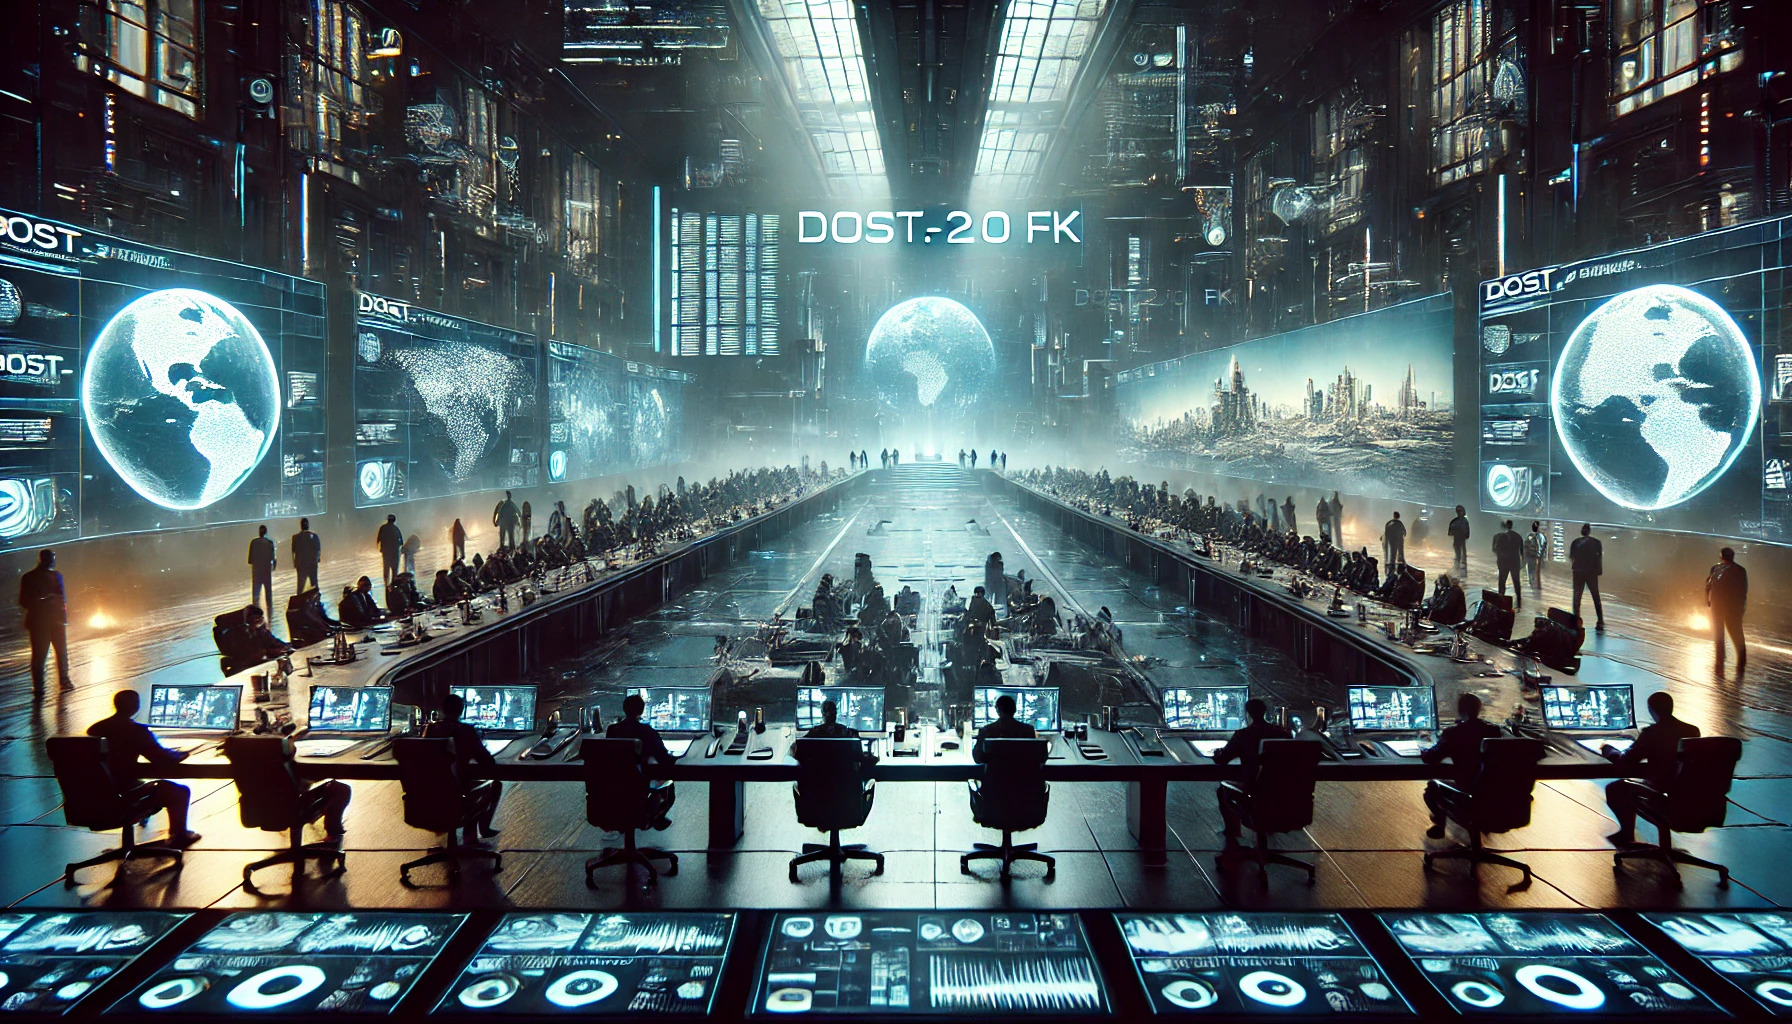
\includegraphics[scale=0.2]{peaceconference-2.jpg}}

\vspace{1.5cm}
\emph{Das Liverollenspiel \ac{dost2} wird vom 07.~bis zum 09.~August 2026
anlässlich fux' 30sten Geburtstag auf Schloss Poggelow stattfinden. Das Spiel
wird von Alex und fux gemeinsam konzeptioniert und in verschiedenen Gruppen
mitgestaltet, ohne, dass die einzelnen Gruppen voneinander wissen. So soll das
Spiel kollektiv entstehen und zugleich für alle ein überraschendes und
hoffentlich gleichermaßen spannendes, ein wenig schauriges aber sicherlich
anregendes Ereignis werden. Wie immer gilt: 24h in-time, high secrecy-level und
schonungslose Immersion. Es lebe die kollektive Revolution!}\\


\squote{Alex und fux, Berlin/Frankfurt, XXI (\ac{nnz})}
